\documentclass{szzclass}
\usepackage{hyperref}

\subject{SI1.2}
\code{BI-WSI-SI-20}
\topic{Přiřazení zodpovědností třídám během návrhu, GRASP vzory (Nízká provázanost, Vysoká soudržnost), popis spolupráce objektů (UML sekvenční diagram, UML diagram tříd - využití během návrhu).}

\begin{document}

\section{Přiřazení zodpovědností třídám během návrhu}
Cílem je správně přiřadit zodpovědnosti třídám.
\begin{itemize}
\item Navrhnout systém tak, aby byl dlouhodobě udržitelný a rozšiřitelný - Rozšíření bude zřejmě provádět jiný tým a není možné se spolehnout na znalosti autorů
\item Snadno lokalizovatelné dopady změn - Snadné odhady pracnosti požadovaných rozšíření
\item Minimalizace dopadů při provádění změn - Změna v jedné části systému by neměla ovlivňovat jinou část
\end{itemize}

\section{GRASP vzory}
\begin{itemize}
\item Základní vzory / principy pro přiřazení zodpovědností třídám
\item Zodpovědnost je úkol, který má třída řešit
\item Existuje mnoho způsobů rozdělení úloh mezi třídy
\item Neexistuje jediné správné řešení
\end{itemize}

\begin{description}
\item[Informační expert] (Information Expert)
\begin{itemize}
\item Základní princip přiřazení zodpovědnosti
\item Popis - Přiřaďte zodpovědnost třídě, která má informace potřebné pro splnění této zodpovědnosti
\end{itemize}
\item[Nízká provázanost] (Low Coupling)
  \begin{itemize}
  \item Zmenšuje dopad při provádění změn
  \item Popis - Přiřaďte zodpovědnost tak, aby provázanost zůstala nízká
  \item Každá třída by si měla vystačit při plnění úkolu sama a minimalizovat nutnost využití ostatních tříd
  \item Zvyšuje možnost znovupoužití
  \item Počet vazeb mezi třídami by měl být minimální
  \end{itemize}
\item[Vysoká soudržnost] (High Cohesion)
  \begin{itemize}
  \item Podporuje nízkou provázanost
  \item Popis - Přiřaďte zodpovědnost tak, aby soudržnost zůstala vysoká
  \item Každá třída by měl být zaměřena na jediný úkol
  \item Zvyšuje srozumitelnost systému
  \item Zodpovědnost třídy je snadno pochopitelná
  \end{itemize}
\end{description}

\begin{itemize}
\item Jedna třída umí všechno
  \begin{itemize}
  \item Nízká provázanost
  \item Malá soudržnost
  \end{itemize}
\item Každá třída pouze jednu metodu
  \begin{itemize}
  \item Vysoká provázanost
  \item Velká soudržnost
  \end{itemize}
\end{itemize}

\section{Popis spolupráce objektů}
\subsection{UML sekvenční diagram}
\begin{itemize}
\item Objekt
  \begin{itemize}
  \item Pojmenovaný
  \item Nepojmenovaný
  \end{itemize}
\item Třída
  \begin{itemize}
  \item Statická metoda
  \end{itemize}
\end{itemize}

\begin{figure}[ht!]
\centering
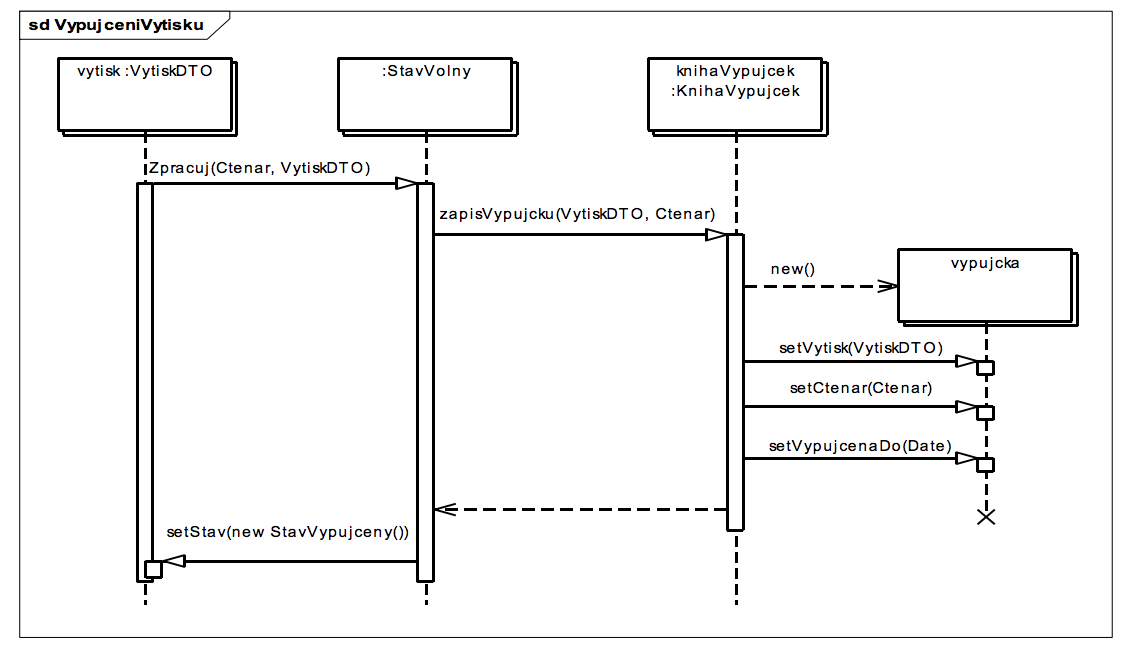
\includegraphics[width=.55\linewidth]{topics/bi-wsi-si-20/images/sekvencni-diagram.png}
\caption{Sekvenční diagram}
\end{figure}

\begin{figure}[ht!]
\centering
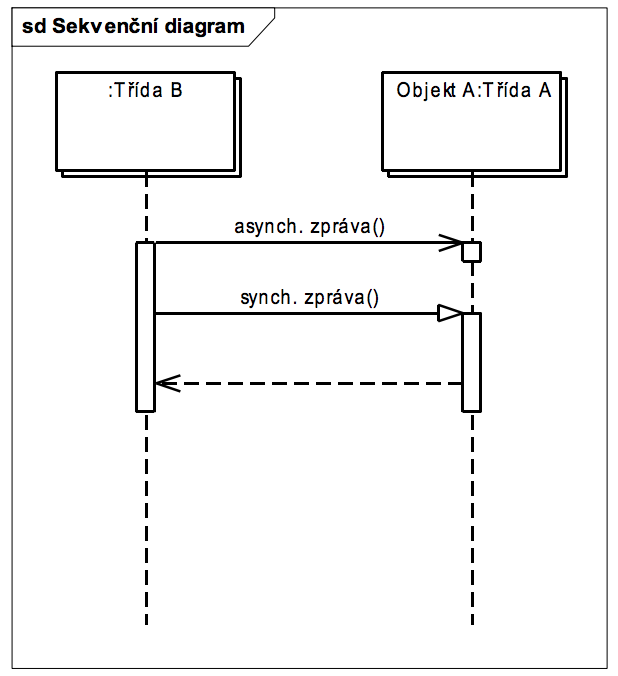
\includegraphics[width=.55\linewidth]{topics/bi-wsi-si-20/images/sekvencni-async.png}
\caption{Zpráva - Asynchronní, Synchronní}
\end{figure}

\begin{figure}[ht!]
\centering
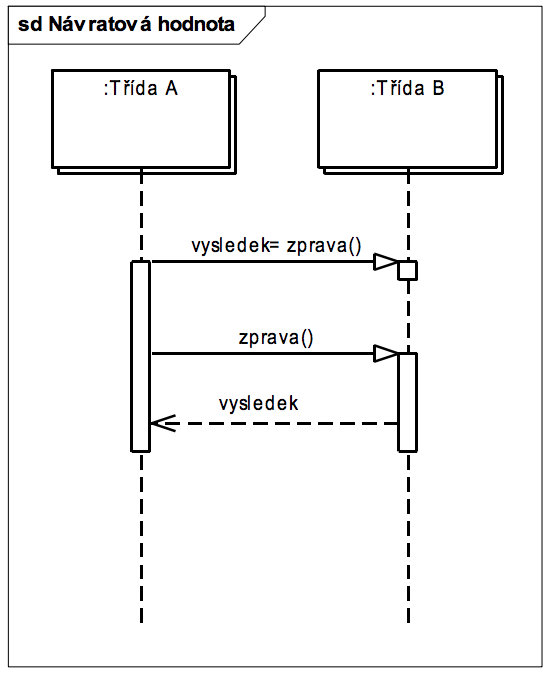
\includegraphics[width=.55\linewidth]{topics/bi-wsi-si-20/images/sekvencni-navratova.png}
\caption{Návratová hodnota - 2 různé způsoby}
\end{figure}

\begin{figure}[ht!]
\centering
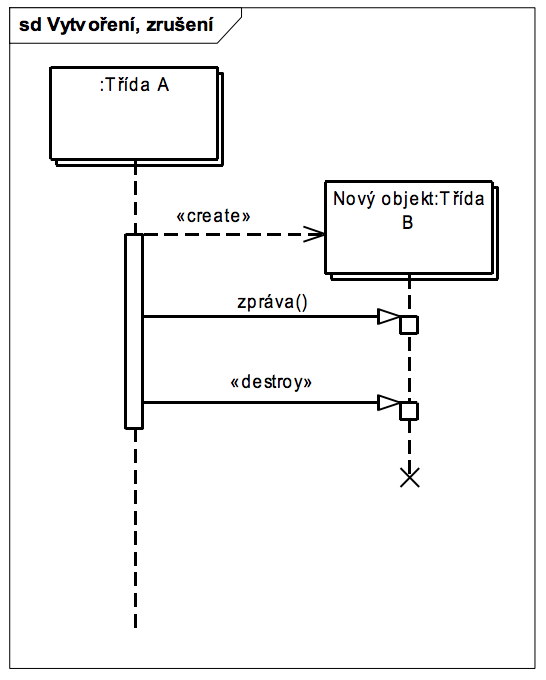
\includegraphics[width=.55\linewidth]{topics/bi-wsi-si-20/images/sekvencni-vytvareni.png}
\caption{Vytvoření a zrušení objektu}
\end{figure}

\subsection{UML diagram tříd - využití během návrhu}
Použití v dokumentaci a pro generování kódů. Může vycházet z doménového návrhu. Diagram tříd je závislý na:
\begin{itemize}
\item Zvolené technologii
\item Zvolené architektuře
\item Použitých architektonických vzorech (GRASP, GoF)
\end{itemize}

\section{Zdroje}
\begin{itemize}
\item Přednášky - \url{https://courses.fit.cvut.cz/BI-SI1/@B171/lectures/index.html}
\end{itemize}

\end{document}
